\chapter{Introduction}
\label{introduction}

\section{Motivation}
\label{intro_motivation}
Folding clothes is a common and necessary, but tedious, task for humans. Additionally, due to the increasing aging of the world population, a growing need exists for robots to be able to help us with laundry.
However, working with non-rigid objects such as clothes is a difficult task for robots, due to the complexity of modeling and manipulating deformable, thin objects. Clothes can be easily entangled when doing laundry, and recognizing individual garments and their category just from color or depth image analysis becomes an almost impossible task, due to occlusions amongst the cluttered clothes. Another challenging aspect when working with deformable objects is how to bring the object into a known configuration from an arbitrary initial state.

\warning{(Move this to "State of the art")}
The pipeline for folding clothes followed throughout robotic literature is based on how it is performed by humans. This allows these tasks to be executed in the same environments as humans, aiming towards a fully-automated or collaborative fashion. Garments are extracted from the washing or drying machine forming a pile, and an iterative process begins. First, an individual clothing article is picked from the pile. Then, the garment is extended in the air or assisted by a flat surface, during which unfolding and wrinkle removing procedures may be performed for aiding the posterior classification and manipulation of the garment. A classification procedure is applied to fit clothing article within a certain garment category. Finally, a standard manipulation sequence specific to its category is applied to fold the garment for storage. This iterative process is repeated until there are no clothes left on the pile.

\begin{figure}[htbp]
    \centering
    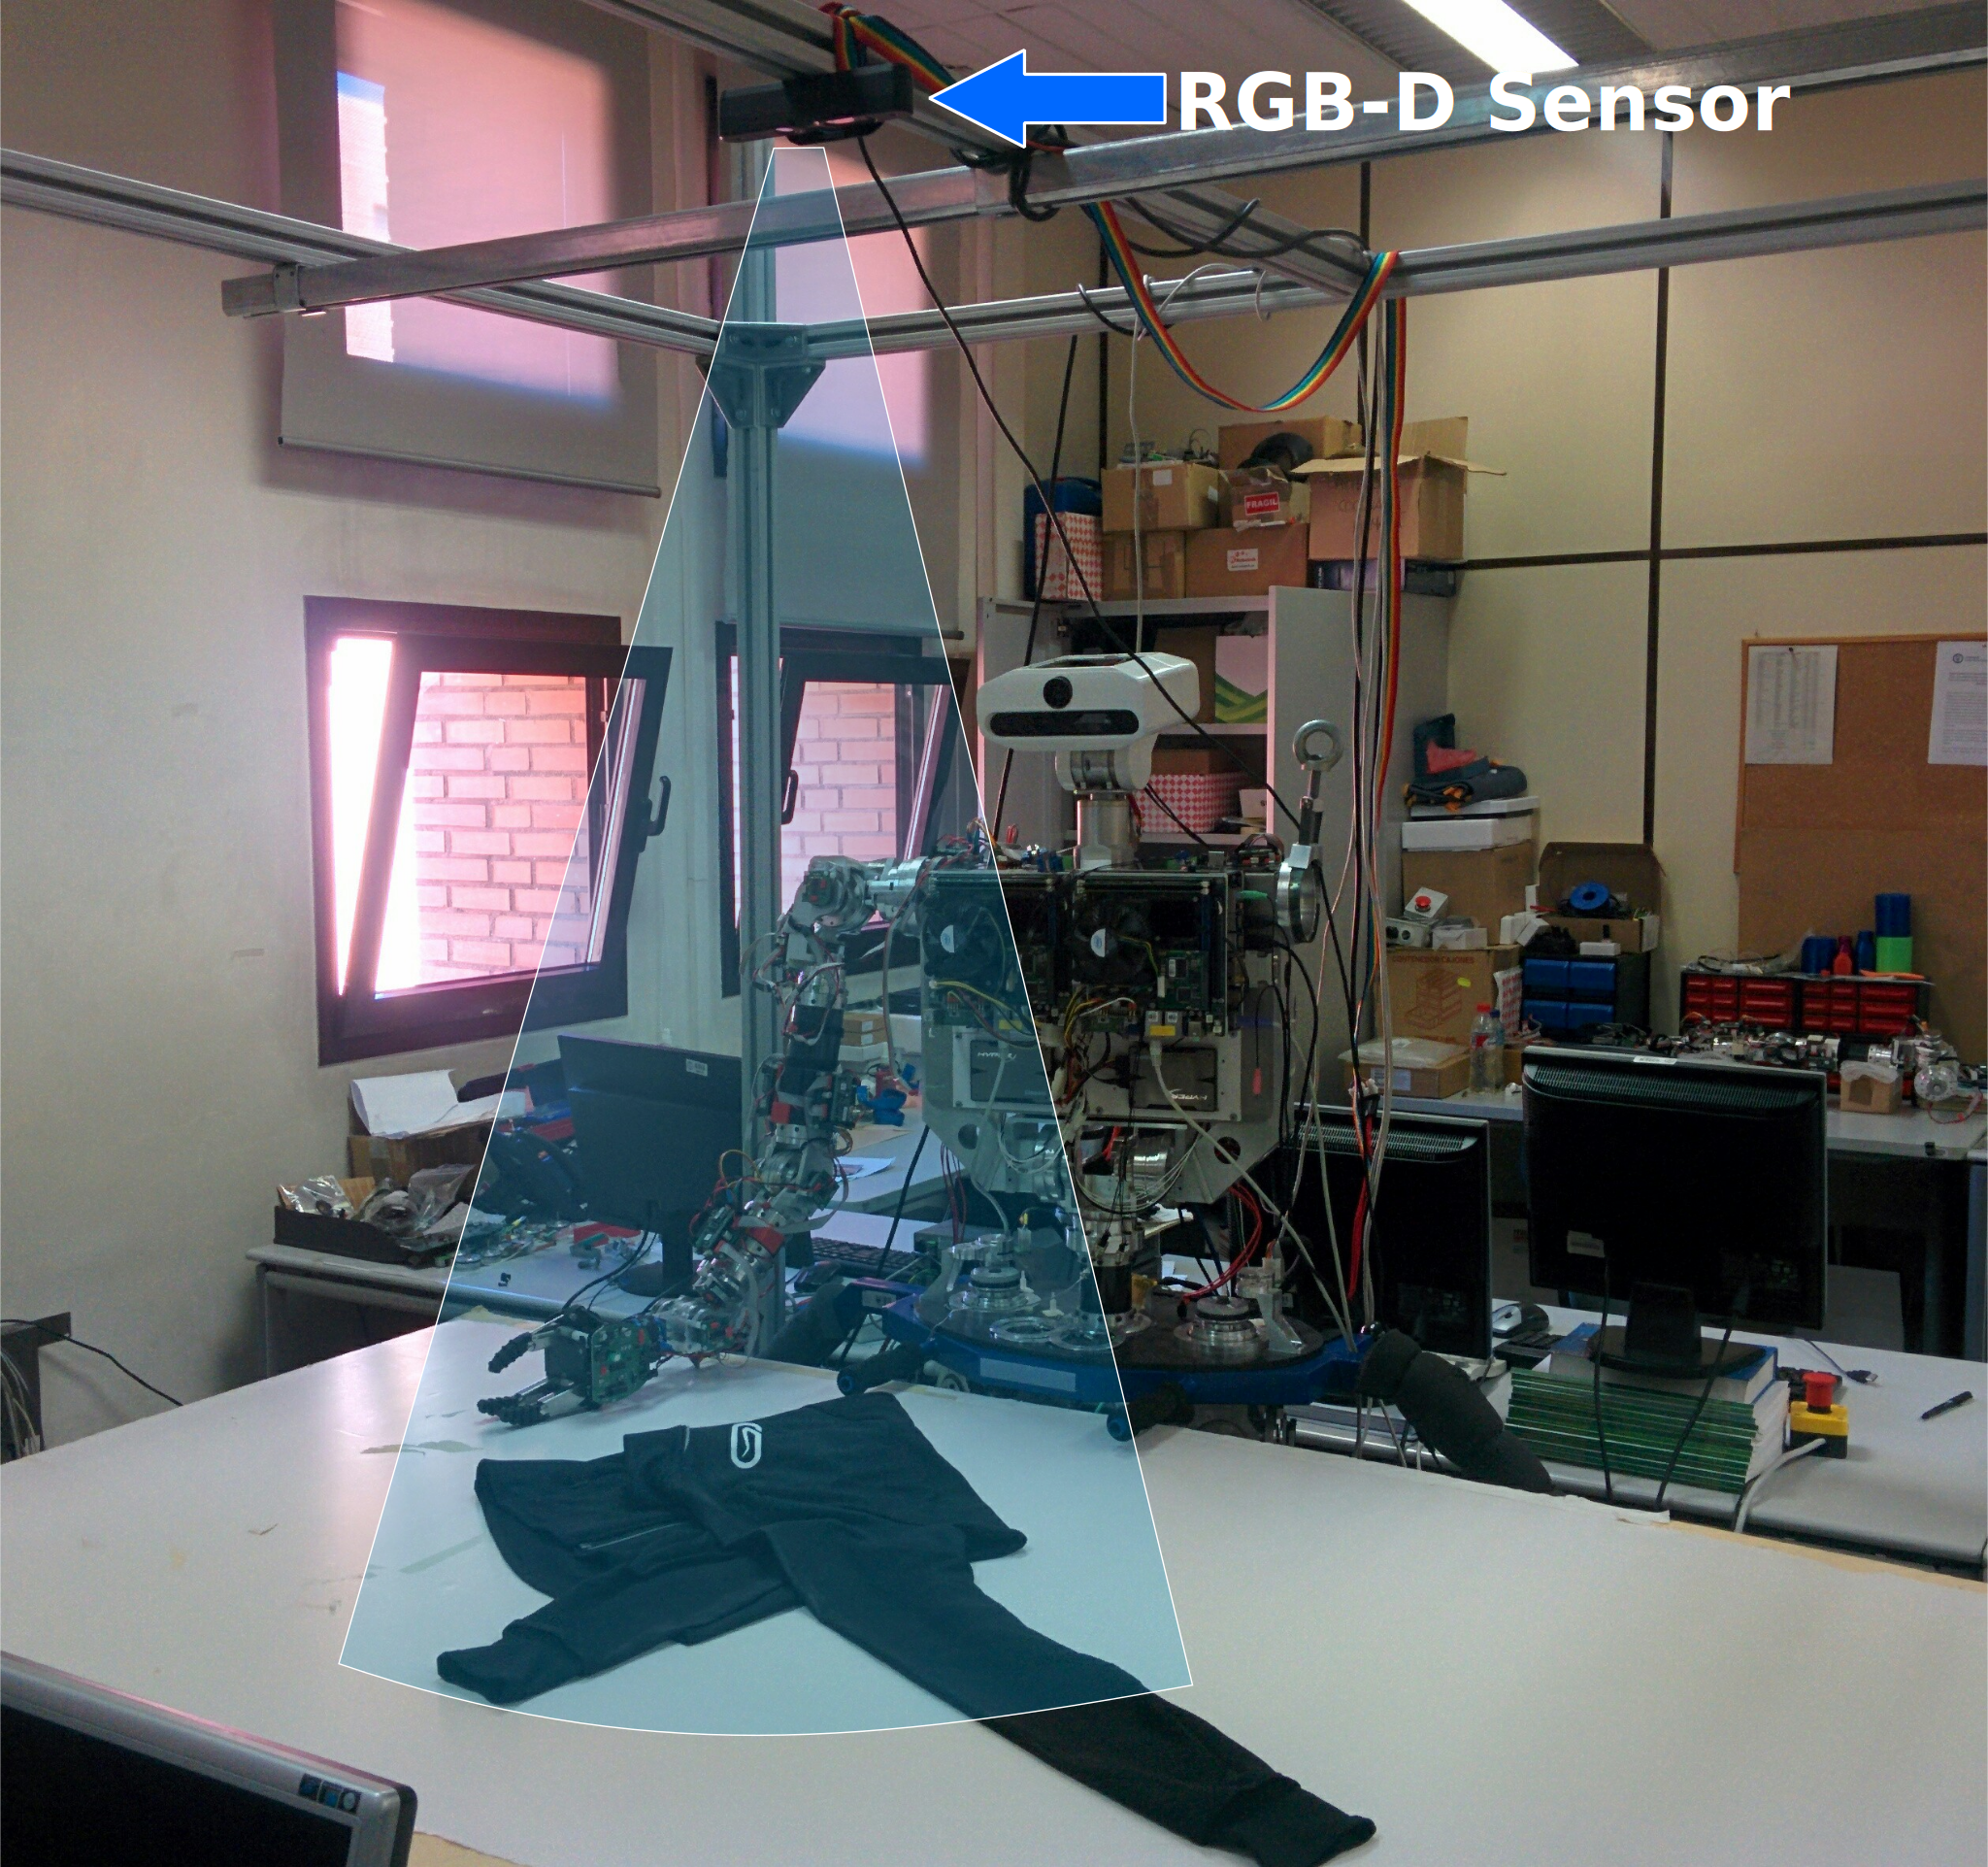
\includegraphics[width=0.45\textwidth]{figures/setup.pdf}
    \caption{Humanoid robotics clothes folding scenario. The clothes are placed on a flat white table while a RGB-D sensor is positioned on the top.}
    \label{setup}
\end{figure}

It is assumed that a clothing article has already been separated from the rest of the clothes to be folded, and placed on a flat surface. The garment could have been placed on that surface either by a robot or by a human coworker, allowing a collaborative folding pipeline in which a human and a robot can perform different parts of the folding process.
As our algorithm is not based on a geometrical model of the garment to be unfolded, it is general enough to be used with any category of garment, from towels and blankets to trousers or shirts, and with any number of folds. 

Our approach consisted in using a depth image from a single point of view to find regions of the garment overlapping other regions, which we considered to be folds. Then, we studied all the possible candidate paths to determine the unfolding direction. 

\section{Objectives}
\label{intro_objectives}
\comment{(Move this to "Motivation"?)}
Extensive work can be found in literature about automated clothes folding once the garment category has been identified, as well as for modeling the garment for fold/wrinkle removal or selecting the most suitable grasping point/strategy. For this reason, this work focuses on how to unfold a clothing article that has been picked up from a pile of clothes and is placed on a flat surface.

The main objective pursued in this work is to develop an algorithm that can estimate the grasping and release points for a deformable object so that a manipulator robot can iteratively unfold a garment for determining its garment category and the folding sequence to apply.

The aforehead mentioned algorithm should also fullfil the following criteria:

\begin{itemize}
	\item It should provide a general method of detecting folds in deformable objects without a prior model of the garment to be unfolded.
	\item It should be able to estimate the best position of the grasping point, direction of movement, and release point in order to unfold the detected fold.
	\item It should rely as little as possible in color or patterns present in the garment, to be independent from the illumination.
\end{itemize}

This system has been tested with thick pieces of cloth such as towels and blankets. These results can be extrapolated to thinner garments provided the depth sensor provides sufficient resolution.

\section{Structure}
\label{intro_structure}

The structure of this document is the following. Chapter \ref{state_of_the_art} provides an overview of the current state of the different methods and techniques to achieve \comment{robot cloth folding}. In chapter \ref{architecture}, the actual algorithm is presented. Chapter \ref{experiments_and_results} is dedicated to introduce the experimental setup, describe the experiments performed and analyze the results obtained. Finally, some conclusions and lines of future work are presented in chapter \ref{conclusions_and_future_work}.